\documentclass[a4paper, 12pt]{article}[abntex2]
\input{cabeçalho}
\usepackage{graphicx} % Required for inserting images
\title{Projeto final - PDPD}
\author{matheus Sevilha dejol}
\date{May 2024}
\usepackage{caption}
\usepackage{float}
\usepackage[alf]{abntex2cite}
\usepackage{titlesec}
\setcounter{secnumdepth}{4}
\newcounter{subsubsubsection}[subsubsection]
\renewcommand\thesubsubsubsection{\thesubsubsection.\arabic{subsubsubsection}}

\begin{document}
    
    %Remove numeração da página atual
    \thispagestyle{empty}

    % Cabeçalho
    \begin{tabular}[l]{ll}
        \multirow{5}*{
\includegraphics[width=50pt]{figuras/logo.png}} & 
        \textbf{\resizebox{!}{0.3cm}{Fundação Universidade Federal do ABC}}\\&
        \textbf{\resizebox{!}{0.3cm}{Pró reitoria de pesquisa}} \\
        & \textbf{\resizebox{!}{0.25cm}{Av. dos Estados, 5001, Santa Terezinha, Santo André/SP, CEP 09210-580}}\\
        & \textbf{\resizebox{!}{0.25cm}{Bloco L, 3ºAndar, Fone (11) 3356-7617}}\\
        & \textbf{\resizebox{!}{0.25cm}{iniciacao@ufabc.edu.br}} \\
    \end{tabular}
    \\
    \\
    \\
    \\
    \\
    \\
    \\
    \\
    \\
    \\
    \\
    \\
    \\
    \\
    \\
    \begin{flushright}
        Relatório final de Inicição Científica\\ 
        referente ao edital: 07/2023-PDPD\\-Pesquisando
        desde o primeiro dia.\vspace{1.5cm} 
    \end{flushright}
    \begin{flushleft}
        \textbf{Nome do aluno:} Matheus Sevilha Dejol\\[1\baselineskip]
        \textbf{Assinatura do aluno:}\\[2\baselineskip]
        \textbf{Nome do orientador:} Marcelo Tanaka Hayashi\\[1\baselineskip]
        \textbf{Assinatura do orientador:}\\[2\baselineskip]
        \textbf{Título do projeto:} Desenvolvimento de código computacional para seleção e dimensionamento de paraquedas utilizados na recuperação de foguetes\\[1\baselineskip]
        \textbf{Palavras chave do projeto:} \\[1\baselineskip]
        \textbf{Área do conhecimento do projeto:} Engenharia aeroespacial, aerodinâmica\\[1\baselineskip]
        \textbf{Bolsista:} Sim, bolsa de iniciação científica do programa PDPD
    \end{flushleft}

    \newpage
    %Sumário
    \tableofcontents

    \newpage
    %Comando para determinar espaçamento entre linhas (1,5 nesse caso)
    \onehalfspacing
        {
        \section{Resumo}
            A utilização de um sistema de recuperação eficiente é crucial para viabilizar economicamente o lançamento de foguetes. Atualmente, a UFABC Rocket Design realiza o processo de seleção e dimensionamento do paraquedas utilizado nesse sistema analisando cada tipo individualmente, o que torna esta etapa do projeto uma tarefa árdua e lenta. Este projeto tem por objetivo desenvolver um código computacional, em linguagem Python, que dimensiona os tipos catalogados de paraquedas para uma dada missão, facilitando a escolha do projetista por uma solução ideal.
        \section{Introdução}
            Atualmente os foguetes permitem o envio de de seres vivos ou objetos ao espaço e seu retorno a terra em segurança. Para chegar em tal ponto, foram necessários mais de 2.000 anos de estudo \cite{Shearer08}\par Apesar desse desenvolvimento, contribuidores de diversos lugares do mundo se mantém buscando novas descobertas para melhoria das tecnologias espaciais já existentes. A inserção de muitos jovens que participam desse processo, se dá pelas competições de foguetimodelismo, como é o caso dos universitários da Rocket Desing, as quais requerem a aplicação de conceitos teóricos e testes práticos para o desenvolvimento de mini-foguetes.\par Mini-foguetes podem ser classificados como foguete modelo e foguete experimentais (Marchi, 2018), sendo a principal diferença entre esses, a restrição dos foguetes-modelo à motores de combustão sólida.
            \\
            \begin{figure}[h!]
                \centering
                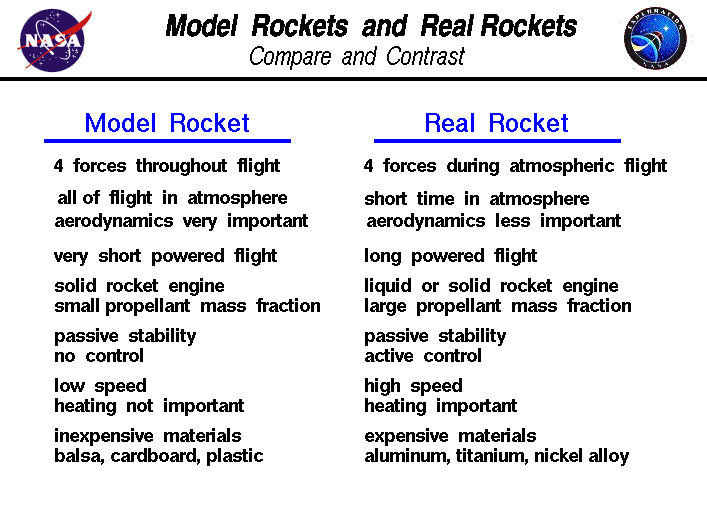
\includegraphics[width = 0.5\linewidth]{figuras/rktcompare.png}
                \caption{Comparativo entre um foguete real e um foguete modelo}
                \caption*{Fonte:(Imagens públicas NASA)}
                \label{fig: model rocket x real rocket}
            \end{figure}
            \par
            Tipicamente, o lançamento de seus foguetes pode ser dividido em quatro etapas propulsionada; balística; de atuação do sistema de recuperação; e de descida lenta \cite{cristello17}. A última delas é resultado do acionamento de um paraquedas, que reduz a velocidade de descida do foguete, de modo a evitar (ou, ao menos, reduzir as chances) que o mesmo seja danificado ao atingir o solo e possibilite a recuperação do protótipo lançado. Esse dispositivo é fundamental para tornar os lançamentos mais viáveis economicamente.
            \\
            \begin{figure}[h!]
                \centering
                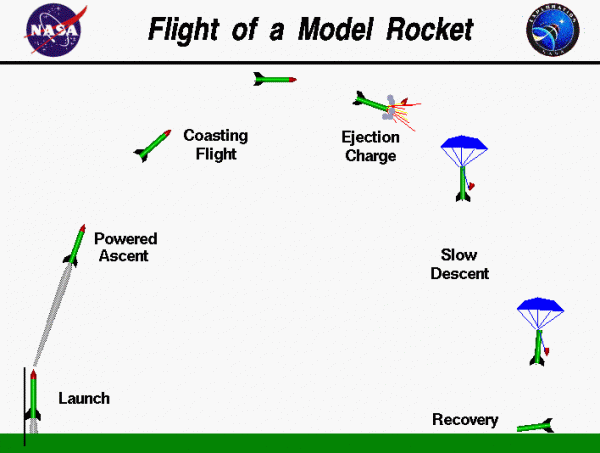
\includegraphics[width = 0.5\linewidth]{figuras/flight.png}
                \caption{Etapas do lançamento de um foguete modelo}
                \caption*{Fonte:(Imagens públicas NASA)}
                \label{fig: etapas do lançamento}
            \end{figure}
            \par Atualmente, a equipe seleciona tipos de paraquedas adequados para uma determinada missão por avaliações bastante subjetivas para, então, os dimensionar. Na busca por um modo mais eficiente de se determinar as possíveis geometrias de paraquedas a serem utilizadas em cada situação, idealizou-se desenvolver um código computacional que realizasse esse trabalho. Dessa forma, seria possível apresentar ao projetista os diversos tipos de paraquedas catalogados e suas respectivas dimensões, para que atendam aos requisitos de projeto, através de um Diagrama de Pareto. Tal procedimento possibilitaria a avaliação do espaço de projeto de uma maneira mais completa, permitindo assim uma escolha mais racional do sistema de recuperação.
        \section{Objetivo}
            O objetivo deste projeto é desenvolver e implementar um código computacional capaz de apresentar formatos e dimensões de paraquedas que atendam as necessidades de uma dada missão. Dessa maneira, possibilitar que a UFABC Rocket Design realize escolhas de maneira mais objetiva e eficaz.
        \section{Fundamentação Teórica}
        O paraquedas é um dos principais componentes para a proteção do foguete, pois é responsável por garantir uma velocidade segura durante o impacto com o solo \cite{miranda21}. Portanto, seu dimensionamento e seleção são etapas críticas no projeto e devem ser realizadas de maneira criteriosa \cite{knacke92} para assegurar o sucesso da missão.
        \par Uma maneira de otimizar esses processos é desenvolver um algoritmo para dimensionamento e seleção de geometrias, implementando-o em um sistema computacional automatizado.
            \subsection{Aerodinâmica de Um Paraquedas}
                \subsubsection{Forças atuando em um corpo no ar} 
                    Tanto corpos em movimento no ar quanto corpos fixos pelos quais o ar se move experimentam forças decorrentes da pressão do ar. No caso dos paraquedas, que são estruturas simétricas, desconsiderando rajadas de vento laterais, a única força significativa sofrida é o arrasto, que atua na direção oposta ao movimento do paraquedas.\cite{knacke92}
                    \\
                     \begin{figure}[h!]
                        \centering
                        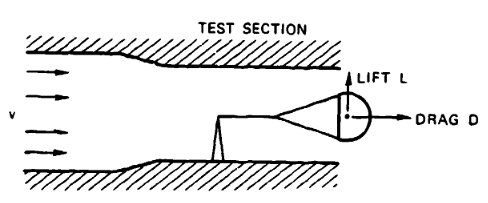
\includegraphics[width = 0.5\linewidth]{figuras/image.png}
                        \caption{Paraquedas em um túnel de vento experienciando a força de arrasto}
                        \caption*{Fonte:(Knacke; Theo W., 1992) }
                        \label{fig: arrasto tunel de vento}
                    \end{figure}
                    \begin{equation}
                         D = q*S*C_D\\
                    \end{equation}
                    \begin{equation}
                        q = \frac{1}{2}*\rho_{ar}*v^2
                    \end{equation}
                    \\
                    $D \rightarrow$ Arrasto\\
                    $q \rightarrow$ Pressão dinâmica do ar\\
                    $S \rightarrow$ Área de projeção do paraquedas\\
                    $C_D \rightarrow$ Coeficiente de arrasto\\
                    $\rho_{ar} \rightarrow$ Densidade do ar\\
                    $v \rightarrow$ Velocidade do ar ou do objeto que se move por ele
                \subsubsection{Equilibrio em Uma Descida Estável}
                    Para um objeto em queda livre, há um determinado momento em que a força de arrasto se iguala a força peso, dessa forma o objeto tem uma resultante nula e adquire uma taxa de descida estável.\par Devido a variação da densidade do ar, a taxa de descida diminui conforme o objeto se aproxima da superfície, porém para taxas menores que $60m/s$ tal fato pode ser desconsiderado\cite{knacke92}.\par
                    Portanto:
                    \begin{equation}
                        D_T = W_T
                    \end{equation}
                    $D_T \rightarrow$ Arrasto total\\
                    $W_T \rightarrow$ Peso total\\
                    \\
                    \begin{equation}
                        D_p + D_f = W_p + W_f
                    \end{equation}
                    
                    \begin{flushleft}
                    $D_P \rightarrow $Arrasto do paraquedas\\
                    $W_p \rightarrow $Peso do paraquedas\\
                    $D_f \rightarrow $Arrasto do foguete\\
                    $W_f \rightarrow $Peso do foguete\\
                    \end{flushleft}
                    \vspace{1.5cm}
                \subsubsection{Dimensionamento}
                    Na maioria dos casos o arrasto gerado pela carga é desprezível em relação ao gerado pelo paraquedas. \cite{knacke92}
                    \begin{equation}
                        D_p = W_p + W_f
                    \end{equation}
                    \par Nesse contexto, o peso do paraaquedas também é tratado como desprezível.\cite{miranda21}
                    \begin{equation}
                        D_p = W_f
                    \end{equation}
                    \begin{equation}
                        \frac{1}{2}*\rho_{ar}*v^2*S*C_D = W_f
                    \end{equation}
                    \\
                    \par Dessa forma, reorganizando a equação 7, podemos definir a área de projeção do paraquedas.\\
                    \begin{equation}
                        S = \frac {2*W_f}{\rho_{ar}* v^{2} * C_D }
                    \end{equation}
                    \\
            \subsection{Critérios para Seleção de Uma Geometria}
                Para projetar o sistema de recuperação, se faz necessário o entendimento do seu objetivo e necessidades, além disso, possuir um claro critério de escolha.\cite{knacke92}\par 
                A confiabilidade do paraquedas é o fator mais importante na tomada de decisão, esse fator é referente ao conhecimento que se possui sobre o comportamento na prática de cada geometria, o qual pode ser adquirido por meio de testes, em túnel de vento, ou queda livre a partir de uma altura conhecida, por exemplo.\cite{knacke92}\par
                A seleção dos paraquedas, geralmente, se inicia levando em conta a estabilidade. Para situações onde são necessários altos níveis de establidade, é adequado a escolha de certas geometrias (nesses casos, geralmente, a maioria dos paraquedas de alto coeficiente de arrasto são descartados).\cite{knacke92}\par
                Além desses, o ceficiente de arrasto também é determinante na escolha de um paraquedas, já que este está diretamente relacionado a taxa de descida. Uma geometria com alto coeficiente de arrasto provê uma determinada taxa de descida a partir de uma área menor do que em relação a um paraquedas com um coeficiente baixo. Dessa forma, geometrias com altos coeficientes permitem obter um determinado arrasto, a partir de áreas menores.\cite{knacke92}\par
                Existem ainda diversos fatores a serem considerados para uma análise precisa da eficiência de uma geometria, como o processo de inflação, a tensão das cordas que prendem o paraquedas, o spill hole, entre outros. No entanto, para os fins deste projeto, apenas os fatores mencionados serão analisados, sendo suficientes para fornecer uma base sólida para a avaliação.
    
            \subsection{Programação}
                A lógica de programação é necessária para quem deseja desenvolver sistemas e programas. A partir dela que é possível definir a sequência lógica de um programa.\cite{costaalgoritmos}.
                \subsubsection{Algoritmos}
                   Os algoritmos são formalmente definidos como um conjunto ordenado de passos executáveis, não ambíguos, que definem um processo finalizável.\cite{sousa2014introduccao}.\par
                    Existem três tipos de algoritmo: descrição narrativa, fluxograma e pseudocódigo.\par
                    A descrição narrativa consiste em escrever os passos para a resolução de um problema a partir de uma linguagem natural, por exemplo, em português.\par
                    Já o fluxograma é o método de exibição dos passos a serem executados por meio de símbolos gráficos predefinidos.\par
                    \vspace{1cm}
                    \begin{figure}[h!]
                        \centering
                        \includegraphics[width = 0.5\linewidth]{figuras/Fluxograma.png}
                        \caption{Exemplo de fluxograma}
                        \caption*{Fonte:(COSTA et al., )}
                        \label{fig: fluxograma}
                    \end{figure}
                    \vspace{1cm}
                    \par Por fim, o pseudocódigo, também chamado de português estruturado, se baseia na escrita de um passo a passo por meio de regras pré-definidas. 
                \subsubsection{Python}
                    Atualmente, vivencia-se um mundo impulsionado pela tecnologia, no qual sistemas computacionais são amplamente utilizados para a coleta e o processamento de dados.\cite{vasiliev2022python}.\par A linguagem de programação Python, caracterizada por sua facilidade de entendimento, destaca-se como a escolha ideal para acessar, manipular e obter insights a partir de dados de qualquer natureza.\cite{vasiliev2022python}.\par
                    O Python dispõe de um conjunto robusto de estruturas para operações básicas, além de bibliotecas open-source (disponibilizadas de forma gratuita) para a manipulação de dados. Entre essas bibliotecas, a Pandas é amplamente reconhecida como o padrão dominante para aplicações Python orientadas a dados.\par 
                    Esta biblioteca fornece estruturas de dados e funções de alto nível, projetadas para tornar intuitivo e flexível o trabalho com dados estruturados ou estruturas tabulares\cite{mckinney2018python}.O Pandas trabalha com duas estruturas de dados principais: a Series, que utiliza uma base unidimensional, e o DataFrame, que utiliza uma base bidimensional.
                    \cite{vasiliev2022python}.
                \subsubsection{Normalização de Dados}
                    A normalização é essencial em diversos algoritmos, permite que os recursos sejam analisados de maneira equânime durante a análise. Sem a normalização, os dados com valores maiores acabam tendo maior peso, mas não necesseriamente contribuem mais para o conjunto dos dados.\cite{zheng18-normalização}.
                    
                    
                    

                
        
        
            
            
            
            
                
                
                    
                
                
                
                
                
                

                
                    
            

            
%Referências bibliográficas 
\bibliography{bibliografia.bib}
\end{document}